\usetikzlibrary{calc}


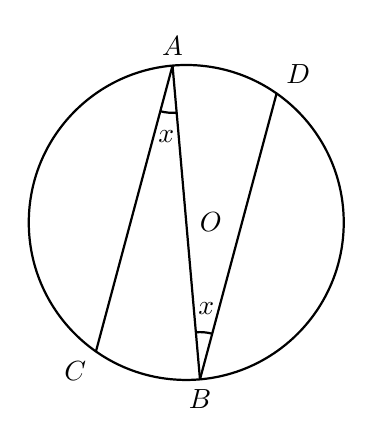
\begin{tikzpicture}[scale=1]

    % Define the center of the circle
    \coordinate (O) at (0,0);

    % Draw the main circle with radius 2
    \draw[thick] (O) circle (2);

    % Define points on the circle
    % A and B form a diameter but are slightly tilted as shown in the image
    \coordinate (A) at (95:2);
    \coordinate (B) at (275:2);
    
    % Define points C and D to create the intersecting chords
    % Angles are chosen to maintain the equal alternating angles 'x' (~20 degrees)
    \coordinate (C) at (235:2);
    \coordinate (D) at (55:2);

    % Draw the line segments (chords)
    \draw[thick] (A) -- (B);
    \draw[thick] (A) -- (C);
    \draw[thick] (B) -- (D);

    % Draw the arc for angle x at A (between chord AC and AB)
    % The angle of line AC is 255 degrees, and AB is 275 degrees from point A
    \draw[thick] (A) ++(255:0.6) arc (255:275:0.6);

    % Draw the arc for angle x at B (between chord BD and AB)
    % The angle of line BD is 75 degrees, and BA is 95 degrees from point B
    \draw[thick] (B) ++(75:0.6) arc (75:95:0.6);

    % Add the labels for the points exactly as shown in the image
    % Using math mode ($...$) ensures English letters render properly
    \node[above] at (A) {$A$};
    \node[below] at (B) {$B$};
    \node[below left] at (C) {$C$};
    \node[above right] at (D) {$D$};

    % Label for the center O, placed slightly to the right of the chord AB
    \node[right] at (0.05, 0) {$O$};

    % Add the angle labels 'x'
    % Placed symmetrically inside the corresponding angles using coordinate calculations
    \node at ($(A) + (265:0.9)$) {$x$};
    \node at ($(B) + (85:0.9)$) {$x$};

\end{tikzpicture}